\chapter{Cosmology: RNS with Gravitation}\label{ch:cosmology}

\small
\begin{quote} According to the \emph{Perfect Cosmological Principle}, 
the Universe on a large scale looks the same everywhere and at all times.
(Fred Hoyle)
\end{quote}
\begin{quote} The thermodynamic properties of self-gravitating
systems are still unclear...The tendency of increasing granularity with time
(in a self-gravitating system), so important to the structure and development 
of the Universe, seems to represent a fundamental principle. 
(Paul Davies \cite{davies})
\end{quote}
\begin{quote} 
GRAVITATION: The universal property of all material objects
to attract each other.\\
GRAVITON: A hypothetical particle which, when passing
to and fro in virtual form bewteen two masses, in large numbers,
is thought to mediate the gravitational attraction between them.
(Guillemin \cite{guillemin})
\end{quote}
\normalsize

\normalsize

\section{Euler's Equations with Gravitation}

The Euler equations including gravitational forces from the mass distribution
can be viewed as a basic (non-relativistic) \emph{cosmological model}.  
We thus consider an inviscid perfect gas 
enclosed in a volume $\Omega$ in $\bbR^3$ with boundary $\Gamma$
(or the whole of $\bbR^3$), over a time interval $I=(0,1]$, assuming 
that the gas is subject to a gravitational force $\nabla\varphi$, where
$\varphi$ is a \emph{gravitational potential} 
coupled (at each time instant) to the mass distribution $\rho$  
through Poisson's equation $\Delta\varphi =\rho$
with (for simplicity) $\varphi =0$ on $\Gamma$. This is a 
\emph{self-gravitating system} since the gravitational force depends
on the mass-distribution  

Replacing $\rho$ by $\Delta\varphi$, we are led to the following version
of Euler's equations with gravitation:  
Find $\hat u=(\varphi ,m,e)$ 
depending on $(x,t)\in Q\equiv \Omega\times I$ such that
\begin{equation}\label{eulergrav}
\begin{array}{rcl}
\Delta\dot\varphi +\nabla\cdot m &=&  0 \quad \mbox{in } Q, \\
\dot m +\nabla\cdot (mu) +\nabla p-\rho\nabla\varphi&=&  0 \quad \mbox{in } Q, \\
\dot e +\nabla\cdot (eu)+p\nabla\cdot u &=& 0  \quad \mbox{in } Q,\\ 
u\cdot n&=&0\quad \mbox{on } \Gamma\times I\\
\varphi &=&0\quad \mbox{on } \Gamma\times I\\
\hat u(\cdot ,0)&=&\hat u^0\quad \mbox{in } \Omega , 
\end{array} 
\end{equation}
where $u=\frac{m}{\Delta\varphi}$, 
$p=(\gamma -1)e$ with $\gamma >1$, and we normalize the gravitational
constant to unity.

\section{The Hen and the Egg}

An interesting aspect of this model with the gravitational
potential $\varphi$ as a primary variable and the mass distribution
$\rho$ as a derived quantity, is that it does not include
\emph{action at distance} in the same way as the conventional model
with $\varphi$ derived from $\rho$ through Poisson's equation 
$\Delta\varphi =\rho$. Instead we have to deal
with the new equation $\Delta\dot\varphi +\nabla\cdot m =0$,
still containing the Laplacian.

Considering the equation $\Delta\varphi =\rho$ as defining
$\varphi$ in terms of $\rho$ or vice versa, of course connects
to which comes first: the egg or the hen. 

Choosing (in an exam for example) 
to explain either how a hen can lay an egg
or how an egg can develop into a hen, you may go for the first
option as appearing to be (somewhat) simpler to deal with.
The idea would be that it would be advantageous to
choose the more complex object of the 
potential/hen rather than the simpler mass/egg, as 
the primary unknown which will come out by solving the equations,
(by some form of computation).
Thus the more complex object, the potential/hen will 
be ``created by computation'' in front of our eyes, thus relieving us
from \emph{explaining} how a mass/egg can create a potential/hen. 
But doing so we have to deal with 
the equation $\Delta\dot\varphi +\nabla\cdot m=0$
expressing ``mass conservation'' in a non-standard form,
which  admittedly seems to involve action at distance if we rewrite it in the form.
$\dot\varphi +(\Delta )^{-1}\nabla\cdot m=0$ for the purpose
of explicitly updating $\varphi$ by time-stepping. What can we do 
to allow time-stepping without inverting the Laplacian?

\section{Perturbed Mass Conservation} 

Well, we may consider
to perturb the equation for mass conservation
$\Delta\dot\varphi +\nabla\cdot m=0$ into: 
\[
\kappa\ddot\varphi -  \Delta\dot\varphi -\nabla\cdot m=0
\]
with $\kappa$ a small positive constant, now allowing time stepping
without inverting the Laplacian. Of course, you could regularize the
equation $\Delta\varphi =\rho$ similarly into  
$\kappa\dot\varphi -\Delta\varphi =\rho$ keeping mass conservation in the
standard form $\dot\rho +\nabla\cdot (\rho u)=0$. In any case,
(\ref{eulergrav}) with $\varphi$ instead of $\rho$ and a perturbed
equation for mass conservation, is a model without action at distance.


\section{Gravitons?}

Solving Poisson's equation $\Delta\varphi =\rho$
equation for the gravitational
potential $\varphi$ in terms of the density $\rho$, reflect that
(somehow) a mass distribution ``creates'' its own gravitational field
(seemingly infinitely fast). The physics of this creation of a hen out
of an egg in the form of
a gravitational potential/force from a mass distribution, is unknown: A
conjecture is that the gravitational field is 
established through an \emph{exchange} of certain hypothetical particles 
called \emph{``gravitons''}. But no gravitons have been detected despite
intense search.



The reverse question is how a hen can lay an egg 
or how a gravitational potential can ``create'' a mass.
A potential with a sharp peak of the form 
$\frac{1}{4\pi\vert x-\bar x\vert}$, would then represent a
unit mass at position $\bar x$.  
In this perspective a tendency of ``mass lumping'' from 
very small initial density
variations, is to be expected from the fact that application of the Laplacian
may enhances variations and thus create positive and negative peaks/masses
out of nothing, with masses of different equal signs attracting each other
and masses with different signs repelleing each other. Our Universe
with positive masses would thus have a twin Universe with negative masses.

In this model, it is thus the gravitational 
potential $\phi$, which is given initially
and which evolves in time (together with momentum and energy)
and from which the mass density $\rho$ is generated by $\Delta\phi =\rho$
in a local ``creation process''.
We here avoid action at distance and we also get a hint
to the possible nature of all the ``dark mass'' seemingly required to account 
for the observed gravitational forces on cosmic scales, as 
mollified potential peaks not strong enough to 
``create visible mass'', but yet having gradients and exerting
gravitational forces.

%The alternative model (\ref{cosmology2}) with $\delta >0$ is a wave equation 
%with finite speed of propagation depending on $\delta$. The proper choice
%of $\delta$ from physical point of view is unclear, while 
%we expect certain outputs to be insensitive to the choice of $\delta$.

\section{The 2nd Law with Gravitation}

The 2nd Law with gravitation takes the form
\begin{equation}
\dot K=W-D+ P,\quad \dot E=-W+D,\quad D>0,
\end{equation}
where 
\[
\begin{split}
P&=-\int_\Omega \rho\nabla\varphi\cdot u\, dx =+\int_\Omega \varphi\nabla\cdot m\, dx=-\int_\Omega\varphi\dot\rho\, dx= \dot\Phi,\\
\Phi &=-\frac{1}{2}\int_\Omega \varphi\Delta\varphi\,dx =\frac{1}{2}\int_\Omega\vert\nabla\varphi\vert^2\, dx.
\end{split}
\] 
By summation, we have
\[
\frac{d}{dt}(K+E -\Phi)=0
\]
stating that the total energy, the sum of
kinetic, heat and gravitational energy $K+E -\Phi$, is conserved.

\section{Irreversibility and Heat Death}

A natural scenario is to start with a hot compressed gas at rest, which is
let free to expand in a \emph{Big Bang} with $W-D-P>0$ setting the
gas in motion until $W-D-P<0$ and $K=0$, whereupon the gas
contracts by gravitation back to a hot compressed state in a \emph{Big Crunch}
allowing the process to start all over with a new Big Bang.

In each cycle of this process some kinetic energy would irreversibly
be transformed into heat energy, which ultimately could lead to 
a stationary state with $W=D$ and $P=0$, a \emph{heat death}. But the 
whole process may have many cycles....and so there may have been Worlds
and intelligent cultures including thermodynamics  
even before the Big Bang of the World we happen to live in...   

\section{A Self-Gravitating Gas in a Box}

To probe the thermodynamics of (\ref{eulergrav}) concretely we solve a
discrete form on a cubic grid filling a box $\Omega =[0,1]^3$, in conservation
form for the density $\rho$, the momentum $m=\rho u$ and the internal energy
density $e$, with the ideal-gas closure
\begin{equation}\label{closure}
p=(\gamma -1)e=\rho T,\qquad \gamma >1,
\end{equation}
so that $T=p/\rho$ is the temperature and $\gamma$ the adiabatic index. The
self-gravitation is supplied through the \emph{mean-subtracted} Poisson coupling
\begin{equation}\label{jeansswindle}
\Delta\varphi = G\,(\rho -\bar\rho ),\qquad
\bar\rho =\frac{1}{\vert\Omega\vert}\int_\Omega\rho\, dx,
\end{equation}
with $\varphi =0$ on $\Gamma$, where $G>0$ is the \emph{gravitational coupling}
(playing the role of $4\pi G_{\mathrm{Newton}}$) and $\bar\rho$ the mean density.

The subtraction of $\bar\rho$ is essential and is the classical
\emph{Jeans swindle}. A strictly uniform gas in a \emph{finite} box is not
force-free if $\rho$ itself sources $\varphi$: with $\varphi =0$ on $\Gamma$ the
solution of $\Delta\varphi =G\rho$ bulges in the interior, so a net inward force
develops everywhere and the whole box \emph{breathes} in and out --- an artifact
of the boundary rather than of any structure in the gas. Sourcing $\varphi$ from
the density \emph{contrast} $\rho -\bar\rho$ makes the uniform background exactly
force-free, so that only departures from uniformity gravitate. This is precisely
what one wants of a cosmological model: it is the \emph{granularity}, not the
mean, that drives the dynamics.

The model so written has exactly \emph{two} control parameters: the
gravitational coupling $G$ and the adiabatic index $\gamma$. Everything in the
competition between collapse and dispersal is decided by these two, as we now
show.

\section{Pressure versus Gravitation: the Jeans Criterion}

Linearize (\ref{eulergrav}), (\ref{closure}), (\ref{jeansswindle}) about a
uniform state $\rho =\bar\rho$, $u=0$, $T=\bar T$ at rest. Writing the density
perturbation as $\delta\rho$ and eliminating $m$ and $\varphi$ one obtains the
wave equation
\begin{equation}\label{waveeq}
\ddot{\delta\rho}=c_s^2\,\Delta(\delta\rho)+G\bar\rho\,\delta\rho,
\qquad c_s^2=\gamma\,\frac{\bar p}{\bar\rho}=\gamma\bar T,
\end{equation}
where $c_s$ is the adiabatic sound speed. For a plane wave
$\delta\rho\propto\exp(i(k\cdot x-\omega t))$ this gives the
\emph{Jeans dispersion relation}
\begin{equation}\label{dispersion}
\omega^2=c_s^2k^2-G\bar\rho=\gamma\bar T\,k^2-G\bar\rho .
\end{equation}
The first term, from pressure, is \emph{stabilizing} (it grows with $\gamma$);
the second, from gravitation, is \emph{destabilizing} (it grows with $G$). A
perturbation grows --- the gas \emph{collapses} --- precisely when
$\omega^2<0$, i.e.\ when
\begin{equation}\label{jeanscrit}
G\bar\rho>\gamma\bar T\,k^2
\qquad\Longleftrightarrow\qquad
\lambda>\lambda_J=2\pi\sqrt{\frac{\gamma\bar T}{G\bar\rho}}\, ,
\end{equation}
$\lambda_J$ being the \emph{Jeans length}. Below the Jeans length pressure wins
and the perturbation merely oscillates as a sound wave ($\omega^2>0$); above it
gravity wins and the perturbation grows.

The decisive observation is that the onset of collapse depends on $G$ and
$\gamma$ \emph{only through the ratio} $G/\gamma$: at a fixed scale $k$ and
fixed background $(\bar\rho ,\bar T)$, doubling the coupling $G$ has exactly the
same effect as halving the stiffness $\gamma$. The dimensionless number that
decides everything is
\begin{equation}\label{jeansnumber}
J=\frac{G\bar\rho}{\gamma\bar T\,k^2},
\qquad\text{collapse}\iff J>1 .
\end{equation}

In a box of side $L$ the longest available wavelength is $\lambda\approx L$, so
structure forms \emph{at all} only if $\lambda_J\lesssim L$, that is
\begin{equation}\label{boxthreshold}
G\gtrsim (2\pi)^2\,\frac{\gamma\bar T}{\bar\rho\,L^2}.
\end{equation}
For $\gamma =2$ and $\bar T=\bar\rho =L=1$ this requires $G\gtrsim 79$; for a
seed of size $\sim L/3$ the threshold is about nine times larger. Below it the
box is Jeans-stable at \emph{every} scale and any initial lump simply pulsates.
This is why a modest coupling produces only an oscillation and never a collapse:
$G$ has not been pushed past the Jeans threshold set by $\gamma$.

\section{Collapse to a Stable Configuration: the Role of $\gamma$}

The Jeans criterion (\ref{jeanscrit}) decides whether collapse \emph{begins}.
Whether the collapse \emph{ends} in a stable, finite lump --- rather than
running away to a singular spike --- is a separate question, and it is decided
by $\gamma$ \emph{alone}, independently of $G$.

Consider a self-gravitating polytropic cloud of fixed mass $M$ and radius $R$.
Under adiabatic compression $p\propto\rho^\gamma$, so the internal energy
density scales as $e\propto\rho^\gamma\propto R^{-3\gamma}$ and the total
internal (thermal) energy as
\[
U=\int_\Omega e\,dx \;\propto\; R^{-3\gamma}\cdot R^3 \;=\; R^{-3(\gamma -1)},
\]
while the gravitational self-energy scales as
\[
W \;\propto\; -\frac{GM^2}{R}\;\propto\; -R^{-1}.
\]
The total energy is therefore $E(R)=A\,R^{-3(\gamma -1)}-B\,R^{-1}$ with
$A,B>0$. As $R\to 0$ the thermal term dominates --- and hence $E$ possesses a
\emph{minimum} at a finite radius, a stable hydrostatic equilibrium --- if and
only if it stiffens faster than gravity, $3(\gamma -1)>1$, that is
\begin{equation}\label{fourthirds}
\boxed{\;\gamma>\tfrac43\;}
\end{equation}
the classical \emph{Chandrasekhar index}. The three regimes are:
\begin{itemize}
\item $\gamma>\tfrac43$: pressure wins under compression; collapse is
\emph{arrested} at a finite quiescent lump, possibly after damped oscillations.
\item $\gamma<\tfrac43$: gravity wins at every compression; collapse
\emph{runs away}, no equilibrium exists.
\item $\gamma=\tfrac43$: the marginal case (governing, e.g., white-dwarf
stability).
\end{itemize}
Thus the two parameters play complementary roles: $G$ (through (\ref{jeanscrit}))
selects \emph{which scales collapse and how fast}, while $\gamma$ (through
(\ref{fourthirds})) decides \emph{whether the collapse can be stopped}. To reach
a stable bound configuration one needs \emph{both} a coupling $G$ large enough
to cross the Jeans threshold \emph{and} a stiffness $\gamma>\tfrac43$ so that the
endpoint is an equilibrium rather than a singularity.

\section{Breathing, Sloshing and Virialization}

These two criteria account for the phenomenology seen in the simulations.

\emph{Breathing.} A uniform gas in which $\rho$ (rather than $\rho-\bar\rho$)
sources $\varphi$ is not in equilibrium in a finite box: it contracts toward the
centre, pressure builds, it rebounds, and the box breathes globally while its
density stays nearly uniform. The Jeans swindle (\ref{jeansswindle}) removes
this boundary artifact, leaving only the genuine gravitational response to
density contrast.

\emph{Sloshing.} A pair of overdensities below the Jeans threshold
($J<1$ at their separation) does not collapse but exchanges mass back and forth
quasi-periodically between the two centres. This is a \emph{virial oscillation}
in the double-well gravitational potential: gas falling toward one centre
overshoots on its pressure and inertia, sloshes to the other, and returns. With
$\gamma>\tfrac43$ and no dissipation the oscillation is undamped, kinetic and
gravitational energy being traded reversibly, $\dot K=P=\dot\Phi$, exactly as in
the energy balance of \S\,\textit{The 2nd Law with Gravitation}.

\emph{Virialization.} To settle into a quiescent lump the gas must \emph{shed}
its infall energy: a stable bound configuration requires dissipation $D>0$ to
convert the ordered kinetic energy of collapse into heat. The entropy so
produced is the irreversible price of structure formation --- the mechanism
behind Davies' ``increasing granularity'' (\S\,\textit{Cosmology}) and behind
the heat death of \S\,\textit{Irreversibility and Heat Death}. Gravitational
structure forms by the conversion, through $D$, of gravitational potential
energy first into bulk motion and then, irreversibly, into heat.

\begin{remark}
In the numerical model the closure is written as $p=\gamma_s\,e$, so that the
adiabatic index is $\gamma=1+\gamma_s$; the stability boundary (\ref{fourthirds})
then reads $\gamma_s>\tfrac13$, and the coupling $G$ is exactly the
$4\pi G_{\mathrm{Newton}}$ of (\ref{jeansswindle}). The two sliders $(G,\gamma_s)$
of the interactive model are precisely the two parameters $(G,\gamma)$ of the
analysis above.
\end{remark}

\section{RNS Simulations of a Self-Gravitating Gas}

We give below some results from RNS solutions of (\ref{eulergrav})
showing the development mass granularity from
uniform mass distributions under expansion.

\begin{figure}[bhpt] 
\centerline{ 
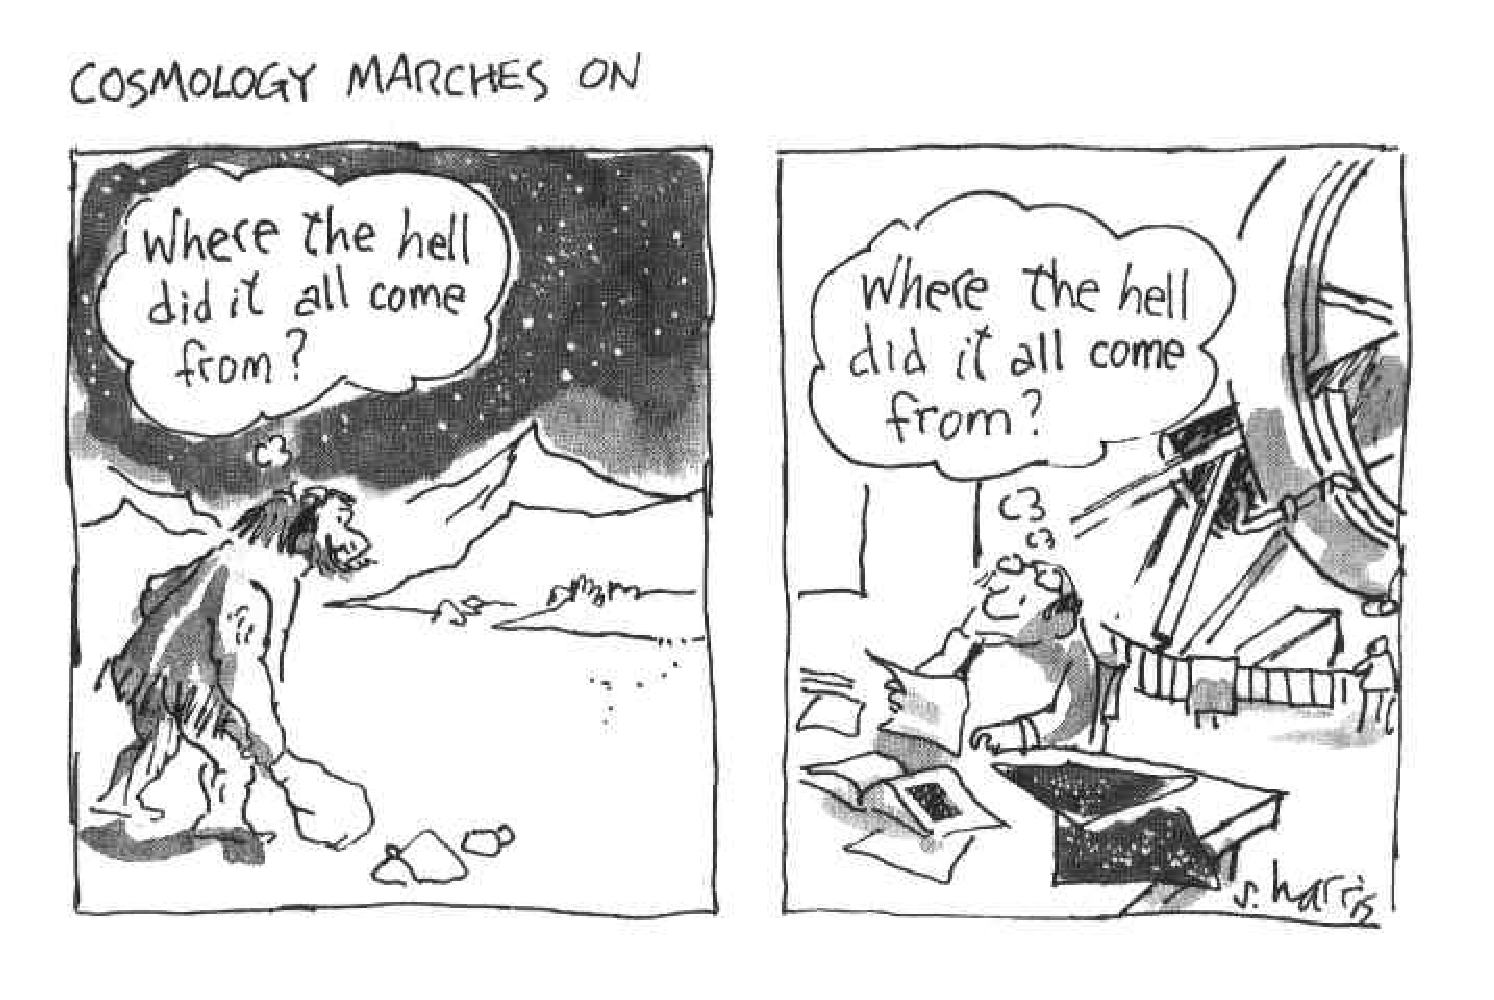
\includegraphics[height=8cm]{ambsthermopict/cosmology.eps} 
} 
\caption{Cosmology theories}
\label{cosmologytheory} 
\end{figure}



\begin{figure}[bhpt]
\centerline{
\includegraphics[height=8cm]{ambsthermopict/cosmology2.eps}
}
\caption{Big Bang expansion}
\label{bigbang2}
\end{figure}

\section{Browser-Runnable 3D RNS-Gravitation Simulator}\label{sec:cosmology_3d_gpu}

A WebGPU companion simulator
\texttt{cosmology\_3d\_gpu\_100.html} is shipped with the
RealMolecule repository
(\texttt{github.com/Claes542/RealMolecule}). It evolves the
self-gravitating RNS system (\ref{eulergrav}) on a $100\times100\times
100$ grid ($10^{6}$ cells) entirely in the browser, using WebGPU
compute shaders for the fluid update and a sub-stepped red-black
Gauss-Seidel relaxation for the Poisson equation $\Delta\varphi = G(\rho - \bar\rho)$.

\paragraph{Initial condition.}
A single Gaussian overdensity at the box centre, both denser and
hotter than the surrounding bath. This is the Big Bang initial
condition of Chapter~\ref{ch:bigbang}: a concentrated hot dense seed
in an otherwise uniform low-density background, with no initial
velocity. The Jeans-swindle source $G(\rho - \bar\rho)$ keeps the
background force-free so that only the density contrast pulls.

\paragraph{Live sliders.}
The simulator exposes the following live controls:
\begin{itemize}
\item \emph{$\gamma$} --- EOS parameter $p = \gamma e = \gamma\rho T$.
\item \emph{Gravity $G$} --- coupling strength.
\item \emph{Seed amp} --- peak overdensity (applied on Reset).
\item \emph{Shock visc $C$} --- shock-viscosity coefficient.
\item \emph{Art visc $\nu$} --- background artificial viscosity.
\item \emph{Seed every} --- particle-trace reset interval.
\item \emph{Trace speed} --- velocity magnification for particle advection.
\item \emph{Fluid substeps/frame} --- numerical resolution in time.
\item \emph{Poisson iters/fluid step} --- gravity convergence.
\end{itemize}

\paragraph{Recommended Big Bang $\to$ Big Crunch settings.}
For a single clean BB$\to$BC cycle followed by a stable virial state:
$G = 500$, seed amp $= 0.5$, $\nu = 1.0$, shock $C = 3.0$, $\gamma = 1$,
Poisson iters $= 10$ or higher for long-time stability.

\paragraph{Reading the display.}
\begin{itemize}
\item \emph{Red particle traces} on the mid-plane: persistent advection
of test particles, redrawn periodically (see \emph{seed every} slider).
During BB the traces radiate outward; during BC they sweep inward;
once virial equilibrium is reached they continue to circulate along
divergence-free streamlines, reflecting the fact that
$\partial_t\rho = 0$ does \emph{not} mean $u = 0$.
\item \emph{Blue polyline} --- density profile $\rho(x_1, x_2^{\mathrm{mid}}, x_3^{\mathrm{mid}})-1$ on the mid-line cross-cut, auto-scaled.
\item \emph{Green polyline} --- temperature profile $T-1$ on the same line.
\item \emph{Cyan polyline} --- gravitational potential $\varphi$ on the same line.
\item \emph{Diagnostic readout} --- peak values of $|\varphi|$, $|\rho-1|$, $|u|$, and simulation time.
\end{itemize}

The simulator is the working companion to the present chapter and
Chapter~\ref{ch:bigbang}: the reader can vary $G$ and the seed amplitude
to scan the Jeans-criterion threshold, watch the
expansion-cooling and compression-warming phases of one Big Bang
followed by one Big Crunch directly in the temperature line plot, and
verify that the cumulative dissipation $D = \int\!\int\mu|\nabla u|^2\,dx\,dt$
prevents the system from oscillating indefinitely.



